%======================================================================
% GMI-03 Tecna struktura.pdf
%======================================================================
% křivka (v originále psací "z" s příčkou)
\providecommand{\gmItrikr}{\mathfrak{z}}
% přeškrtnutý člen (v originále škrtnuto)
\providecommand{\gmItriskrt}[1]{\tikz[baseline=(X.base)]{\node[inner sep=0pt](X){$#1$};\draw[gray](X.south west)--(X.north east);}}
\providecommand{\gmItriskrtb}[1]{\tikz[baseline=(X.base)]{\node[inner sep=0pt](X){$#1$};\draw[gray](X.north west)--(X.south east);}}

\section{Tečná struktura}
\strana{GMI-03-1}

\begin{itemize}[nosep]
  \item Prostor směrů (rychlostí)
  \item Prostor derivací na $\mathcal{F}M$ v bodě
  \item Tečný prostor
  \item Kotečný prostor
  \item Vektorová pole a pole 1-forem
  \item Lieova závorka
\end{itemize}

%----------------------------------------------------------------------
\newpage
\strana{GMI-03-2}
\subsection{Prostor směrů (rychlostí)}

\begin{minipage}{0.62\textwidth}
\kw{parametrizovaná křivka} skrze $x$
\[
  \gmItrikr: I\to M \quad\text{hladké}
\]
\quad $I$ interval v okolí $0$ v $\mathbb{R}$ \\
\quad $\gmItrikr(0) = x$
\end{minipage}
\begin{minipage}{0.36\textwidth}
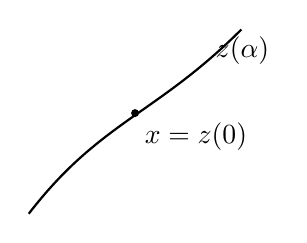
\begin{tikzpicture}[scale=0.9]
  \draw[thick] (0,0) .. controls (1,1.3) and (1.8,1.4) .. (3,2.6);
  \fill (1.5,1.42) circle (1.6pt);
  \node[below right] at (1.5,1.42) {$x = \gmItrikr(0)$};
  \node[right] at (2.5,2.3) {$\gmItrikr(\alpha)$};
\end{tikzpicture}
\end{minipage}

derivace fce podél křivky $\gmItrikr$
\[
  \frac{\dd}{\dd\alpha}\, f\circ\gmItrikr\Big|_{\alpha=0}
\]

křivky stejného směru (rychlosti) \\
\quad $\gmItrikr_1(\alpha)$ a $\gmItrikr_2(\alpha)$ mají stejný směr (rychlost) \\
\quad $\equiv$ \quad $\forall f\in\mathcal{F}M$ \quad
$\dfrac{\dd}{\dd\alpha}f\circ\gmItrikr_1\Big|_{\alpha=0} = \dfrac{\dd}{\dd\alpha}f\circ\gmItrikr_2\Big|_{\alpha=0}$ \\
\quad jedná se o relaci ekvivalence

\begin{definice}[Směr (rychlost)]
\kw{směr} $\equiv$ třída ekviv.\ křivek stejného směru \\
třídu ekv.\ křivce $\gmItrikr$ označíme \quad
$\vzorec{\dot\gmItrikr \equiv \dfrac{D\gmItrikr}{\dd\alpha}\Big|_{\alpha=0}}$
\end{definice}

\begin{vysvetleni}[Směr jako třída křivek]
Na obecné varietě nemáme \uv{šipky} ani rozdíl bodů, takže rychlost křivky nelze definovat jako $\lim(\gmItrikr(\alpha)-\gmItrikr(0))/\alpha$. Místo toho říkáme, že dvě křivky skrz $x$ mají stejný směr, pokud \emph{dávají stejné derivace všem funkcím}. Směr (= tečný vektor v geometrickém pojetí) je pak celá třída takových křivek; symbol $\dot\gmItrikr = \frac{D\gmItrikr}{\dd\alpha}$ označuje třídu, do níž křivka patří (velké $D$ připomíná, že nejde o obyčejnou derivaci čísel). Směr nese i \uv{rychlost běhu} parametru: přeparametrizace $\alpha\to2\alpha$ dá dvojnásobný směr. Viz Krtouš, odd.~2.2 (značí $\frac{D z}{\dd\tau}$, definice D2.2 derivace ve směru).
\end{vysvetleni}

\textbf{derivace ve směru} \\
\quad $a$ směr v $x$ a $\gmItrikr(\alpha)$ jeho reprez.\ $a = \dot\gmItrikr$
\[
  \vzorec{a[f] = \frac{\dd}{\dd\alpha}f\circ\gmItrikr\Big|_{\alpha=0}}
\]
\quad nezávisí na volbě reprezentanta

\textbf{derivace složené fce} \\
\quad $f = F(f^1,\dots,f^k)$ \qquad $f, f^j\in\mathcal{F}M$ \qquad $F:\mathbb{R}^k\to\mathbb{R}$ hladká
\[
  \Downarrow\qquad a[f] = \sum_j \frac{\partial F}{\partial f^j}(f^1,\dots,f^k)\; a[f^j]
\]
\quad plyne z definice převedením na obyčejné derivování

%----------------------------------------------------------------------
\strana{GMI-03-3}
\textbf{komponenty směru} \\
\quad zvolme mapu $(U,[x^i])$ v okolí bodu $x$ \\
\quad směr je jednoznačně určen d-ticí čísel
\[
  \vzorec{a^i \equiv a[x^i]}
\]
\quad tj.\ platí
\begin{align*}
  \frac{\dd}{\dd\alpha}x^i\circ\gmItrikr\Big|_{\alpha=0} &= a[x^i] \qquad\text{pro křivku } \gmItrikr(\alpha) \\
  \Rightarrow\quad \forall f\in\mathcal{F}M \quad \frac{\dd}{\dd\alpha}f\circ\gmItrikr\Big|_{\alpha=0} &= a[f] \\
  \Rightarrow\quad \dot\gmItrikr &= a
\end{align*}

\underline{důkaz} \\
\quad nechť $\bar f = f\circ x^{-1}$ je souř.\ repr.\ fce $f$
\begin{align*}
  \frac{\dd}{\dd\alpha}f\circ\gmItrikr\Big|_{\alpha=0}
  &= \frac{\dd}{\dd\alpha}\bar f\circ x\circ\gmItrikr\Big|_{\alpha=0}
   = \frac{\partial\bar f}{\partial x^j}\circ x\circ\gmItrikr\Big|_{\alpha=0}\,
     \frac{\dd}{\dd\alpha}x^j\circ\gmItrikr\Big|_{\alpha=0} \\
  &\underset{\substack{\uparrow\\ \text{předpoklad}}}{=} \frac{\partial\bar f}{\partial x^j}\,a[x^j]
   \underset{\substack{\uparrow\\ \text{der.\ sl.\ fce ve směru } a}}{=} a[f]
\end{align*}

každá d-tice $a^i$ určuje směr \\
\quad definujme souřadnicovou přímku $l_{a^i}(\alpha)$
\[
  x^i\big(l_{a^j}(\alpha)\big) = x_0^i + \alpha a^i \qquad x_0^i = x^i(x)
\]
\quad komponenty směru $\dot l_{a^j}$ jsou $a^i$
\[
  \dot l_{a^j}[x^i] = \frac{\dd}{\dd\alpha}x^i\big(l_{a^j}(\alpha)\big)\Big|_{\alpha=0} = a^i
\]

\begin{vysvetleni}[Komponenty směru]
Celá informace o směru je obsažena v $d$ číslech $a^i=a[x^i]$ -- derivacích souřadnicových funkcí. Důkaz ukazuje proč: libovolnou $f$ zapíšeme jako funkci souřadnic, $f=\bar f(x^1,\dots,x^d)$, a řetízkové pravidlo převede $a[f]$ na $\frac{\partial\bar f}{\partial x^j}\,a[x^j]$. Naopak každá $d$-tice čísel je realizována \uv{souřadnicovou přímkou} $l_{a^j}$ (přímka v souřadnicích, ne nutně geometricky přímá). Prostor směrů je tedy v bijekci s $\mathbb{R}^d$; tato bijekce ovšem závisí na mapě a při změně souřadnic se komponenty mění Jacobiho maticí $\partial\tilde x^i/\partial x^j$ (kontravariantní transformace).
\end{vysvetleni}

\textbf{změna souřadnic} \\
\quad dvě mapy \quad $(U,[x^i])$ \quad $(\tilde U,[\tilde x^i])$ \\
\quad komponenty směru $\dot\gmItrikr$ $\to$ $a^i$, $\tilde a^i$
\[
  \vzorec{\tilde a^i = \dot\gmItrikr[\tilde x^i] = \frac{\partial\tilde x^i}{\partial x^j}\,\dot\gmItrikr[x^j] = \frac{\partial\tilde x^i}{\partial x^j}\,a^j}
\]

%----------------------------------------------------------------------
\strana{GMI-03-4}
\textbf{lineární struktura prostoru směrů} \\
\quad definujeme sčítání a škálování směrů
\[
  a + b = \dot l_{a^i+b^i} \qquad\qquad \kappa a = \dot l_{\kappa a^i}
\]
\quad kde $a^i$, $b^i$ jsou komponenty $a$, $b$ vůči nějakým souřadnicím \\
\quad nezávisí na volbě souř., tj.
\[
  \underset{\substack{\updownarrow\\ x\text{-komponenty}\\ a^i + b^i}}{\dot l_{a^i+b^i}}
  \;=\;
  \underset{\substack{\updownarrow\\ \tilde x\text{-komponenty}\\ \tilde a^i + \tilde b^i}}{\dot{\tilde l}_{\tilde a^i+\tilde b^i}}
\]
\quad $x$-komponenty $a^i+b^i$ $\longleftrightarrow$ $\tilde x$-komponenty $\tilde a^i+\tilde b^i$: lineární vztah \\
\quad $\to$ \ $\dot l_{a^i+b^i}$ má $\tilde x$-komponenty \
$\dfrac{\partial\tilde x^i}{\partial x^j}(a^j+b^j) = \tilde a^i + \tilde b^i$

\textbf{souřadnicové směry} \\
\quad $\dfrac{\partial}{\partial x^i}$ \quad směr souřadnicové čáry
\[
  x^{-1}(\underbrace{\dots}_{\text{konstanty}}\ \underset{\substack{\uparrow\\ i\text{-tá pozice}}}{\alpha}\ \underbrace{\dots}_{\text{konstanty}})
\]
\[
  \vzorec{\frac{\partial}{\partial x^i}[f] = \frac{\partial\bar f}{\partial x^i}(x)} \qquad\text{kde } f = \bar f\circ x
\]

směry $\dfrac{\partial}{\partial x^i}$ tvoří bázi v prostoru směrů
\[
  \vzorec{a = a^i\frac{\partial}{\partial x^i}} \qquad\text{kde } a^i = a[x^i]
\]
\[
  \Updownarrow\qquad a[f] = a[x^i]\,\frac{\partial\bar f}{\partial x^i} = a^i\frac{\partial}{\partial x^i}[f]
\]

\begin{vysvetleni}[Lineární struktura a souřadnicové směry]
Sčítání směrů se definuje \uv{přes komponenty}: sečteme komponenty a vezmeme směr příslušné souřadnicové přímky. Aby to byla dobrá definice, nesmí výsledek záviset na mapě -- to zaručuje, že transformace komponent $\tilde a^i=\frac{\partial\tilde x^i}{\partial x^j}a^j$ je \emph{lineární} (Jacobiho matice v bodě $x$ je pevná). Symbol $\frac{\partial}{\partial x^i}$ označuje směr $i$-té souřadnicové čáry (mění se jen $x^i$, ostatní souřadnice konstantní) a jako operátor na funkcích dává obyčejnou parciální derivaci souřadnicového vyjádření $\bar f$. Zápis $a=a^i\frac{\partial}{\partial x^i}$ pak říká, že tečný vektor je diferenciální operátor 1.~řádu (Einsteinova sumace přes $i$).
\end{vysvetleni}

%----------------------------------------------------------------------
\newpage
\strana{GMI-03-5}
\subsection{Prostor derivací na $\mathcal{F}M$ v bodě}

\begin{definice}[Derivace v bodě]
$a$ je \kw{derivace funkcí z $\mathcal{F}M$ v bodě $x$} $\equiv$
\[
  a:\mathcal{F}M\to\mathbb{R}
\]
\begin{align*}
  a[\kappa f] &= \kappa\,a[f] &&\qquad f,g\in\mathcal{F}M,\ \kappa\in\mathbb{R} \\
  a[f+g] &= a[f] + a[g] \\
  a[fg] &= a[f]\,g|_x + f|_x\,a[g]
\end{align*}
\end{definice}

\begin{vysvetleni}[Algebraická definice tečného vektoru]
Druhý, čistě algebraický přístup: tečný vektor v $x$ je lineární zobrazení $\mathcal{F}M\to\mathbb{R}$ splňující Leibnizovo pravidlo \emph{vyhodnocené v bodě $x$} (proto $g|_x$, $f|_x$). Žádné křivky ani souřadnice nejsou potřeba. Každá derivace ve směru (předchozí oddíl) tuto definici splňuje; dále se ukáže, že i naopak každá derivace v bodě je derivací ve směru nějaké křivky -- oba přístupy tedy dávají tentýž prostor $\mathbf{T}_xM$.
\end{vysvetleni}

\textbf{lokalita derivace v bodě $x$}
\begin{align*}
  f = 0 \text{ na okolí } x &\quad\Rightarrow\quad a[f] = 0 \\
  f = \text{konst na okolí } x &\quad\Rightarrow\quad a[f] = 0 \\
  f = g \text{ na okolí } x &\quad\Rightarrow\quad a[f] = a[g]
\end{align*}
\underline{důkaz:}
\begin{enumerate}[label=\arabic*), nosep]
  \item nechť $f|_U = 0$, $x\in U$; \ $\operatorname{supp}\beta\subset U$, $\beta(x) = 1$ \quad $\Big\}\Rightarrow\ \beta f = 0$ na $M$
  \[
    0 = a[\beta f] = a[\beta]\,\underbrace{f|_x}_{0} + \underbrace{\beta|_x}_{1}\,a[f] = a[f]
  \]
  \item[3)] $f|_U = g|_U \ \Rightarrow\ (f-g)|_U = 0 \ \Rightarrow\ a[f] = \oprava{a[g]}{g[g]}$
  \item[2)] $a[1^2] = a[1] + a[1] \ \Rightarrow\ a[1] = 0$, \qquad $a[\kappa] = \kappa\,a[1] = 0$ \qquad 3) $\Rightarrow$ stačí na okolí
\end{enumerate}
umožňuje zúžit der.\ na $\mathcal{F}U$, resp.\ na svazek $\mathcal{F}M$ -- viz dále

\begin{vysvetleni}[Lokalita a funkce $\beta$]
$\beta$ je hladká \uv{čepičková} (bump) funkce: rovná se $1$ v bodě $x$ a mimo $U$ je nulová; na hladké varietě vždy existuje. Protože $f=0$ na $U$ a $\beta=0$ mimo $U$, je součin $\beta f$ nulový všude, a Leibnizovo pravidlo pak vynutí $a[f]=0$. Důsledek: $a[f]$ závisí jen na chování $f$ v libovolně malém okolí $x$. Proto lze derivaci v bodě aplikovat i na funkce definované jen na okolí $U$ (např.\ na souřadnice $x^i$, které obecně nejsou globální funkce na $M$) -- to se využívá všude dále.
\end{vysvetleni}

\textbf{derivace složené fce} \\
\quad $f = F(f^1,\dots,f^k)$ \qquad $f^1,\dots,f^k\in\mathcal{F}M$ \qquad $F$ hladká $\mathbb{R}^k\to\mathbb{R}$ \quad $\Rightarrow$
\[
  \vzorec{a[f] = \sum_j\frac{\partial F}{\partial f^j}(f^1,\dots,f^k)\;a[f^j]}
\]
\underline{důkaz:} \\
\quad lineární aprox.\ fce $F$ včetně zbytku (analýza v $\mathbb{R}^k$)
\begin{gather*}
  F(u^1,\dots,u^k) = F(u_0^1,\dots,u_0^k) + \sum_j\frac{\partial F}{\partial u^j}(u_0^1,\dots,u_0^k)\,\Delta u^j + \mathcal{O}(\Delta u^p\Delta u^q) \\
  \Delta u^j = u^j - u_0^j
\end{gather*}
\begin{align*}
  a[f] &= a\Big[f|_x + \sum_j\frac{\partial F}{\partial f^j}(f^1\dots f^k)\Big|_x\big(f^j - f^j|_{x}\big) + \mathcal{O}(\Delta f^p\Delta f^q)\Big] \\
  &= \sum_j\frac{\partial F}{\partial f^j}(f^1,\dots,f^k)\Big|_x\,a[f^j] + \mathcal{O}(\Delta f^p)
\end{align*}
\quad kde $u^j\to f^j$, \ $u_0^j = f^j|_x$

\begin{vysvetleni}[Proč zmizí zbytek]
Konstanta $f|_x$ dá nulu (lokalita, bod 2). Zbytek je součtem členů tvaru $h\,\Delta f^p\Delta f^q$ s hladkou $h$ a $\Delta f^p=f^p-f^p|_x$ (Hadamardovo lemma -- zbytek Taylorova rozvoje lze psát jako hladký násobek součinu přírůstků). Leibniz dává $a[\Delta f^p\Delta f^q]=a[f^p]\,\Delta f^q|_x+\Delta f^p|_x\,a[f^q]=0$, protože $\Delta f^p|_x=0$. Tedy každý člen alespoň druhého řádu v přírůstcích má nulovou derivaci v $x$; zápis \uv{$+\mathcal{O}(\Delta f^p)$} je třeba chápat jako členy úměrné $\Delta f^p|_x=0$. Speciálně pro $F$ = souřadnicové vyjádření $\bar f$ a $f^j=x^j$ dostaneme $a[f]=\frac{\partial\bar f}{\partial x^j}a[x^j]$, tj.\ i algebraická derivace je určena komponentami $a[x^j]$.
\end{vysvetleni}

%----------------------------------------------------------------------
\newpage
\strana{GMI-03-6}
\subsection{Tečný prostor}

\begin{definice}[Tečný prostor $\mathbf{T}_xM$ v bodě $x$]
\[
  \vzorec{\mathbf{T}_xM \equiv \text{prostor derivací v } x}
\]
\kw{tečný vektor} v $x$ $\equiv$ derivace v bodě $x$ \\
lineární struktura
\begin{align*}
  (a+b)[f] &= a[f] + b[f] \\
  (\kappa a)[f] &= \kappa\,a[f]
\end{align*}
\end{definice}

\textbf{vztah ke směrům}
\begin{itemize}
  \item derivace ve směru $\dot\gmItrikr$ v bodě $x$ je derivace na $\mathcal{F}M$ v $x$ \\
        $\dot\gmItrikr[f]$ \quad -- splňuje linearitu a Leibnize
  \item $\dfrac{\partial}{\partial x^i}$ tvoří bázi v $\mathbf{T}_xM$ \\
        nechť $f = \bar f\circ x$ \ $\Rightarrow$ \ $a[f] = \bar f_{,j}\big|_x\,a[x^j] = a[x^j]\,\dfrac{\partial}{\partial x^j}[f]$ \\
        $\Rightarrow$ \ $a = a^j\dfrac{\partial}{\partial x^j}$ \ kde $a^j = a[x^j]$ \ $\Rightarrow$ \ $\dfrac{\partial}{\partial x^i}$ báze
  \item každý tečný vektor je směrem \\
        komponenty $a^i$ tečného vekt.\ $a$ určují souř.\ př.\ $l_{a^i}$ ve směru $\dot l_{a^i}$
\end{itemize}

\pozor{ztotožníme pojem tečného vektoru a směru}

\begin{vysvetleni}[Tečný prostor -- shrnutí]
Oba přístupy (geometrický: třídy křivek; algebraický: derivace v bodě) dávají tentýž $d$-rozměrný vektorový prostor $\mathbf{T}_xM$ se souřadnicovou bází $\frac{\partial}{\partial x^i}$. Dále proto vektor $a$ chápeme zároveň jako \uv{šipku} tečnou ke křivkám i jako operátor $f\mapsto a[f]$. Krtouš (odd.~2.2) obě pojetí jen stručně zmiňuje a používá navíc abstraktní indexy: vektor zapisuje $a^n$, souřadnicový vektor $\frac{\partial^n}{\partial x^j}$ (tento zápis se v poznámkách zatím nepoužívá).
\end{vysvetleni}

\underline{pozn:} značení $\dfrac{\partial}{\partial x^i}$ pro bázový vektor tečný k souř.\ čáře je kontextové, tj.\ $\dfrac{\partial}{\partial x^i}$ závisí na definici všech souřadnic \\
\quad změna $x^j$, $j\neq i$ mění význam $\dfrac{\partial}{\partial x^i}$ \quad $\to$ příklad

%----------------------------------------------------------------------
\strana{GMI-03-7}
značení $\dfrac{\partial}{\partial x^i}$ pro bázi vektorů tečných ke souř.\ čáře je kontextové, tj.\ $\dfrac{\partial}{\partial x^i}$ závisí na def.\ všech souřadnic \\
změna $x^j$, $j\neq i$ mění význam $\dfrac{\partial}{\partial x^i}$

\begin{priklad}[Př: $\mathbb{R}^2$]
\begin{minipage}[t]{0.55\linewidth}
souřadnice $x, y$ \\
souřadnice $\bar x, \bar y$
\begin{align*}
  \bar x &= x & x &= \bar x \\
  \bar y &= y + x & y &= \bar y - \bar x
\end{align*}
vektorové báze
\begin{align*}
  \frac{\partial}{\partial\bar x} &= \frac{\partial x}{\partial\bar x}\frac{\partial}{\partial x} + \frac{\partial y}{\partial\bar x}\frac{\partial}{\partial y} = \frac{\partial}{\partial x} - \frac{\partial}{\partial y} \\
  \frac{\partial}{\partial\bar y} &= \frac{\partial x}{\partial\bar y}\frac{\partial}{\partial x} + \frac{\partial y}{\partial\bar y}\frac{\partial}{\partial y} = \frac{\partial}{\partial y}
\end{align*}
máme tedy
\begin{align*}
  x &= \bar x & &\text{ale} & \frac{\partial}{\partial x} &\neq \frac{\partial}{\partial\bar x} \\
  y &\neq \bar y & &\text{ale} & \frac{\partial}{\partial y} &= \frac{\partial}{\partial\bar y}
\end{align*}
\end{minipage}\hfill
\begin{minipage}[t]{0.42\linewidth}
\centering
\begin{tikzpicture}[scale=0.75,>=Stealth]
  % horní mřížka x,y
  \begin{scope}
    \clip (-0.4,-0.4) rectangle (3.6,3.2);
    \foreach \x in {0,1.2,2.4,3.6} \draw[NavyBlue!50] (\x,-0.4) -- (\x,3.2);
    \foreach \y in {0.2,1.4,2.6} \draw[NavyBlue!50] (-0.4,\y) -- (3.6,\y);
  \end{scope}
  \draw[->,very thick] (1.2,1.4) -- (1.2,2.6) node[left] {$\frac{\partial}{\partial y}$};
  \draw[->,very thick] (1.2,1.4) -- (2.4,1.4) node[below] {$\frac{\partial}{\partial x}$};
  \draw[->] (3.7,0) -- (4.2,0) node[right] {$x$};
  \draw[->] (3.9,3.0) -- (3.9,3.5) node[right] {$y$};
  % dolní mřížka xbar, ybar
  \begin{scope}[yshift=-4.6cm]
    \begin{scope}
      \clip (-0.4,-0.4) rectangle (3.6,3.2);
      \foreach \x in {0,1.2,2.4,3.6} \draw[NavyBlue!50] (\x,-0.4) -- (\x,3.2);
      \foreach \c in {-2.2,-1,0.2,1.4,2.6,3.8,5,6.2} \draw[NavyBlue!50] (-0.4,\c+0.4) -- (3.6,\c-3.6);
    \end{scope}
    \draw[->,very thick] (1.2,1.4) -- (1.2,2.6) node[left] {$\frac{\partial}{\partial\bar y}$};
    \draw[->,very thick] (1.2,1.4) -- (2.4,0.2) node[below] {$\frac{\partial}{\partial\bar x}$};
    \draw[->] (3.7,-0.3) -- (4.2,-0.3) node[right] {$\bar x$};
    \draw[->] (3.6,3.3) -- (4.0,3.7) node[right] {$\bar y$};
  \end{scope}
\end{tikzpicture}
\end{minipage}
\end{priklad}

\begin{vysvetleni}[Proč je $\partial/\partial x^i$ kontextové]
$\frac{\partial}{\partial x^i}$ je derivace podél čáry, na níž se mění $x^i$ a \emph{ostatní souřadnice jsou konstantní}. Změníme-li ostatní souřadnice, změní se i tyto čáry: v příkladu je $\bar x=x$, ale čára \uv{$\bar y=$ konst} je šikmá přímka $y=-x+$konst, takže $\frac{\partial}{\partial\bar x}=\partial_x-\partial_y\neq\partial_x$. Obecně $\frac{\partial}{\partial\bar x^i}=\frac{\partial x^j}{\partial\bar x^i}\frac{\partial}{\partial x^j}$ -- v transformaci figuruje \emph{inverzní} Jacobiho matice, tj.\ parciální derivace starých souřadnic podle nových, a ta závisí na všech nových souřadnicích. Naopak 1-forma $\dd x^i$ (viz dále) závisí jen na funkci $x^i$.
\end{vysvetleni}

%----------------------------------------------------------------------
\strana{GMI-03-8}
\begin{priklad}[Př: $\mathbb{E}^3$, kart.\ souř.\ $x,y,z$, sf.\ souř.\ $r,\vartheta,\varphi$]
\begin{align*}
  x &= r\sin\vartheta\cos\varphi \\
  y &= r\sin\vartheta\sin\varphi \\
  z &= r\cos\vartheta
\end{align*}
transformace souř.\ bází
\begin{align*}
  \frac{\partial}{\partial r} &= \frac{\partial x}{\partial r}\frac{\partial}{\partial x} + \frac{\partial y}{\partial r}\frac{\partial}{\partial y} + \frac{\partial z}{\partial r}\frac{\partial}{\partial z}
   = \sin\vartheta\cos\varphi\frac{\partial}{\partial x} + \sin\vartheta\sin\varphi\frac{\partial}{\partial y} + \cos\vartheta\frac{\partial}{\partial z} \\
  &= \frac{x}{r}\frac{\partial}{\partial x} + \frac{y}{r}\frac{\partial}{\partial y} + \frac{z}{r}\frac{\partial}{\partial z}
   \hspace{4cm} r = \sqrt{x^2+y^2+z^2} \\[4pt]
  \frac{\partial}{\partial\vartheta} &= \frac{\partial x}{\partial\vartheta}\frac{\partial}{\partial x} + \frac{\partial y}{\partial\vartheta}\frac{\partial}{\partial y} + \frac{\partial z}{\partial\vartheta}\frac{\partial}{\partial z}
   = r\cos\vartheta\cos\varphi\frac{\partial}{\partial x} + r\cos\vartheta\sin\varphi\frac{\partial}{\partial y} - r\sin\vartheta\frac{\partial}{\partial z} \\
  &= z\frac{x}{\varrho}\frac{\partial}{\partial x} + z\frac{y}{\varrho}\frac{\partial}{\partial y} - \varrho\frac{\partial}{\partial z}
   \hspace{3.2cm} \varrho = r\sin\vartheta = \sqrt{x^2+y^2} \\[4pt]
  \frac{\partial}{\partial\varphi} &= \frac{\partial x}{\partial\varphi}\frac{\partial}{\partial x} + \frac{\partial y}{\partial\varphi}\frac{\partial}{\partial y} + \frac{\partial z}{\partial\varphi}\frac{\partial}{\partial z}
   = -r\sin\vartheta\sin\varphi\frac{\partial}{\partial x} + r\sin\vartheta\cos\varphi\frac{\partial}{\partial y} \\
  &= -y\frac{\partial}{\partial x} + x\frac{\partial}{\partial y}
\end{align*}
inverzní vztahy
\begin{align}
  x\frac{\partial}{\partial x} + y\frac{\partial}{\partial y} + z\frac{\partial}{\partial z} &= r\frac{\partial}{\partial r} \tag{1}\\
  x\frac{\partial}{\partial x} + y\frac{\partial}{\partial y} - \frac{\varrho^2}{z}\frac{\partial}{\partial z} &= \oprava{\frac{\varrho}{z}\frac{\partial}{\partial\vartheta}}{\frac{\partial}{\partial\vartheta}} \tag{2}\\
  -y\frac{\partial}{\partial x} + x\frac{\partial}{\partial y} \hspace{1.75cm} &= \frac{\partial}{\partial\varphi} \tag{3}
\end{align}
\begin{align*}
  \frac{\partial}{\partial z} &= \frac{z}{r}\frac{\partial}{\partial r} - \frac{\varrho}{r^2}\frac{\partial}{\partial\vartheta} && \Leftarrow\ (1) - (2) \\
  x\frac{\partial}{\partial x} + y\frac{\partial}{\partial y} &= \frac{\varrho^2}{r}\frac{\partial}{\partial r} + \frac{z\varrho}{r^2}\frac{\partial}{\partial\vartheta} && \Leftarrow\ \square(1) + \square(2) \qquad (4) \\
  \frac{\partial}{\partial x} &= \frac{x}{r}\frac{\partial}{\partial r} + \frac{xz}{\varrho r^2}\frac{\partial}{\partial\vartheta} - \frac{y}{\varrho^2}\frac{\partial}{\partial\varphi} && \Leftarrow\ (4) - (3) \\
  \frac{\partial}{\partial y} &= \frac{y}{r}\frac{\partial}{\partial r} + \frac{yz}{\varrho r^2}\frac{\partial}{\partial\vartheta} + \frac{x}{\varrho^2}\frac{\partial}{\partial\varphi} && \Leftarrow\ (4) + (3)
\end{align*}
\end{priklad}

\begin{vysvetleni}[Jak číst inverzi]
Vztah (2) vznikne vynásobením výrazu pro $\frac{\partial}{\partial\vartheta}$ faktorem $\varrho/z$ (proto správně $\frac{\varrho}{z}\frac{\partial}{\partial\vartheta}$ vpravo; s tímto faktorem pak sedí i všechny další řádky). Zápis $\square(1)+\square(2)$ znamená lineární kombinaci s vhodnými koeficienty, konkrétně $\frac{\varrho^2}{r^2}(1)+\frac{z^2}{r^2}(2)$, kdy se vyruší člen s $\partial_z$; podobně $\partial_x=\frac{x}{\varrho^2}(4)-\frac{y}{\varrho^2}(3)$ a $\partial_y=\frac{y}{\varrho^2}(4)+\frac{x}{\varrho^2}(3)$. Výsledek je tentýž jako použití inverzní Jacobiho matice, $\frac{\partial}{\partial x}=\frac{\partial r}{\partial x}\partial_r+\frac{\partial\vartheta}{\partial x}\partial_\vartheta+\frac{\partial\varphi}{\partial x}\partial_\varphi$. Pozor: $\partial_\vartheta$, $\partial_\varphi$ nejsou jednotkové (mají velikost $r$, resp.\ $\varrho$) -- souřadnicová báze není ortonormální.
\end{vysvetleni}

%----------------------------------------------------------------------
\strana{GMI-03-9}
\subsubsection*{Tečný bundle}
\begin{definice}[Tečný bundle]
soubor všech teč.\ vekt.\ ve všech bodech tvoří \kw{tečný bundle}
\[
  \vzorec{\mathbf{T}M = \bigcup_{x\in M}\mathbf{T}_xM}
\]
\end{definice}

tečný bundle je dif.\ varieta \\
\quad atlas indukovaný atlasem na $M$ \\
\quad mapa $(U,x)$ na $M$ \qquad $x\in U$ \\
\quad vektoru $a\in\mathbf{T}_xM$ přiřadíme souřadnice
\[
  x_* = [x^i, a^i] \qquad\text{kde}\qquad x^i = x^i(x) \qquad a^i = a[x^i]
\]
\quad dostáváme mapu $(\mathbf{T}U, x_*)$ na $\mathbf{T}M$ \\
\quad přechodová zobr.\ mezi mapami $(\mathbf{T}U,x_*)$ a $(\mathbf{T}U',x'_*)$
\[
  x_*\circ x'^{-1}_* \qquad \Big[x^i(x'^{-1}),\ \frac{\partial x^i}{\partial x'^j}(x'^{-1})\,a'^j\Big]
\]
\quad kde \quad $a = a^i\dfrac{\partial}{\partial x^i} = a'^i\dfrac{\partial}{\partial x'^i}$ \quad $\Rightarrow$ \quad $a^i = \dfrac{\partial x^i}{\partial x'^j}(x'^{-1})\,a'^j$

\begin{vysvetleni}[Tečný bundle jako varieta]
Bod variety $\mathbf{T}M$ je dvojice (bod $x$, vektor $a\in\mathbf{T}_xM$); má tedy $2d$ souřadnic: $d$ souřadnic bodu a $d$ komponent vektoru. Přechodové zobrazení mezi indukovanými mapami je hladké, protože jde o přechodové zobrazení na $M$ doplněné o lineární transformaci komponent Jacobiho maticí (jejíž prvky jsou hladké funkce bodu) -- proto je $\mathbf{T}M$ hladká varieta dimenze $2d$. Zápis $(x'^{-1})$ znamená, že parciální derivace se vyhodnocují v bodě o čárkovaných souřadnicích. Přirozená projekce $\mathbf{T}M\to M$, $(x,a)\mapsto x$, dělá z $\mathbf{T}M$ vektorový bundle s vlákny $\mathbf{T}_xM$. Fyzikálně: $\mathbf{T}M$ je prostor poloh a rychlostí (konfigurační prostor lagrangeovské mechaniky).
\end{vysvetleni}

%----------------------------------------------------------------------
\newpage
\strana{GMI-03-10}
\subsection{Kotečný prostor $\mathbf{T}^*_xM$}

\begin{definice}[Kotečný prostor]
\kw{kotečný prostor} $\mathbf{T}^*_xM$ $\equiv$ duální prostor k prostoru $\mathbf{T}_xM$ tečných vekt.\ v $x$ \\
$\alpha\in\mathbf{T}^*_xM$ nazýváme \kw{1-forma} -- lin.\ funkcionál na $\mathbf{T}_xM$
\[
  \vzorec{\alpha[a] = \langle\alpha, a\rangle = \alpha\cdot a}
  \qquad\nwarrow\ \text{preferovaný zápis -- zúžení}
\]
\end{definice}

\textbf{reflexivita prostorů $\mathbf{T}_xM$ a $\mathbf{T}^*_xM$} \\
\quad duál k $\mathbf{T}^*_xM$ izomorfní s $\mathbf{T}_xM$ -- ztotožňujeme
\[
  a[\alpha] = a\cdot\alpha = \alpha\cdot a = \alpha[a] \qquad\text{-- zúžení}
\]
\quad plyne z konečné dim.

\textbf{duální báze} \\
\quad $e_i$ \ báze v $\mathbf{T}M$ \\
\quad $e^i$ \ báze v $\mathbf{T}^*M$ \qquad $\vzorec{e^i\cdot e_j = \delta^i_j}$ \ $\leftarrow$ duální báze \\
\quad zúžení v souřadnicích
\[
  \alpha\cdot a = \alpha_i a^i \qquad\qquad \alpha = \alpha_i e^i \qquad a = a^j e_j
\]

\begin{vysvetleni}[1-formy a zúžení]
1-forma je lineární \uv{měřidlo} vektorů: přiřadí vektoru číslo, lineárně. Tečka $\alpha\cdot a$, závorka $\langle\alpha,a\rangle$ a $\alpha[a]$ jsou tři zápisy téže operace -- \emph{zúžení} (kontrakce); poznámky preferují tečku. Protože $\dim\mathbf{T}_xM=d<\infty$, je dvojný duál kanonicky izomorfní s původním prostorem, a proto lze psát i $a\cdot\alpha$ -- zúžení je symetrické. Duální báze $e^i$ je určena podmínkou $e^i\cdot e_j=\delta^i_j$, takže $\alpha_i=\alpha\cdot e_i$, $a^i=e^i\cdot a$. Krtouš (odd.~2.3) píše zúžení abstraktními indexy jako $a^n\alpha_n$. Pozn.: \uv{báze v $\mathbf{T}M$} zde znamená bázi v $\mathbf{T}_xM$.
\end{vysvetleni}

%----------------------------------------------------------------------
\strana{GMI-03-11}
\subsubsection*{Gradient funkce}

derivace ve směru definuje lin.\ funkcionál na teč.\ vektorech \\
\quad $a[f]$ jako funkcionál na $a$ \qquad
$(a+b)[f] = a[f] + b[f]$ \qquad $(\kappa a)[f] = \kappa\,a[f]$
\begin{definice}[Gradient]
\quad $\Downarrow$ \\
existuje 1-forma $\dd f$ -- \kw{gradient $f$} -- taková, že
\[
  \vzorec{a[f] = \langle\dd f, a\rangle = a\cdot\dd f}
\]
\end{definice}

\begin{vysvetleni}[Gradient]
Pro pevnou $f$ je $a\mapsto a[f]$ lineární funkcionál na $\mathbf{T}_xM$, tedy prvek duálu -- to je $\dd f$. Gradient je tedy přirozeně \emph{1-forma}, ne vektor (k převodu na vektor by byla potřeba metrika). V souřadnicích $\dd f=\frac{\partial\bar f}{\partial x^i}\dd x^i$, tj.\ složky gradientu jsou parciální derivace $f_{,i}$. Geometricky: $\dd f$ v bodě $x$ odpovídá \uv{vrstevnicím} $f$ -- vektor tečný k vrstevnici dává $a\cdot\dd f=0$. Viz Krtouš, odd.~2.3, vztah (2.1): $a[f]=a\cdot\dd f=a^n\dd_n f$.
\end{vysvetleni}

vlastnosti gradientu v $x$
\begin{align*}
  \dd(f+g) &= \dd f + \dd g && f,g\in\mathcal{F}M \\
  \dd(\kappa f) &= \kappa\,\dd f && \kappa\in\mathbb{R} \\
  \dd(fg) &= f|_x\,\dd g + \dd f\,g|_x
\end{align*}

derivace složené fce \\
\quad $f = F(f^1,\dots,f^k)$ \qquad $f, f^j\in\mathcal{F}M$ \qquad $F:\mathbb{R}^k\to\mathbb{R}$ hladká
\[
  \Rightarrow\quad \dd f = \sum_j\frac{\partial F}{\partial f^j}(f^1\dots f^k)\,\dd f^j
\]
\quad vše plyne z analog.\ vlastn.\ der.\ ve směru $a[f]$

\textbf{souřadnicové báze v $\mathbf{T}^*_xM$} \\
\quad $\dd x^i$ tvoří bázi v $\mathbf{T}^*_xM$ duální k $\dfrac{\partial}{\partial x^i}$
\[
  \vzorec{\frac{\partial}{\partial x^i}\cdot\dd x^j = \frac{\partial}{\partial x^i}[x^j] = \frac{\partial x^j}{\partial x^i} = \delta^j_i}
\]
\quad \pozor{forma $\dd x^i$ závisí pouze na $x^i$} (nekontextová jako $\dfrac{\partial}{\partial x^i}$)

\textbf{souřadnice vektorů a 1-forem}
\begin{align*}
  \alpha &= \alpha_a\,\dd x^a & \alpha_a &= \alpha\cdot\frac{\partial}{\partial x^a} \\
  a &= a^a\frac{\partial}{\partial x^a} & a^a &= a\cdot\dd x^a
\end{align*}
\quad transformace souřadnic
\begin{align*}
  \dd x'^j &= \frac{\partial x'^j}{\partial x^i}\,\dd x^i & &\Rightarrow & \vzorec{a'^a = \frac{\partial x'^a}{\partial x^b}\,a^b} \\
  \frac{\partial}{\partial x'^j} &= \frac{\partial x^i}{\partial x'^j}\frac{\partial}{\partial x^i} & &\Rightarrow & \vzorec{\alpha'_a = \frac{\partial x^b}{\partial x'^a}\,\alpha_b}
\end{align*}

\begin{vysvetleni}[Souřadnicová báze 1-forem a transformace]
$\dd x^i$ je gradient souřadnicové funkce $x^i$; vztah $\frac{\partial}{\partial x^i}\cdot\dd x^j=\delta^j_i$ říká, že $\{\dd x^i\}$ je duální báze k $\{\frac{\partial}{\partial x^i}\}$. Na rozdíl od $\frac{\partial}{\partial x^i}$ je $\dd x^i$ určena jen samotnou funkcí $x^i$ (v příkladu na str.~GMI-03-7: $\dd\bar x=\dd x$, ač $\partial_{\bar x}\neq\partial_x$). Komponenty získáme zúžením s duální bází: $a^a=a\cdot\dd x^a$, $\alpha_a=\alpha\cdot\frac{\partial}{\partial x^a}$. Odtud transformační zákony: komponenty vektorů se transformují Jacobiho maticí $\partial x'/\partial x$ (\uv{kontravariantně}, horní index), komponenty 1-forem maticí inverzní $\partial x/\partial x'$ (\uv{kovariantně}, dolní index) -- tak, aby $\alpha_a a^a$ bylo na volbě souřadnic nezávislé.
\end{vysvetleni}

%----------------------------------------------------------------------
\strana{GMI-03-12}
\subsubsection*{Kotečný bundle}
\begin{definice}[Kotečný bundle]
soubor všech 1-forem ve všech bodech tvoří \kw{kotečný bundle}
\[
  \vzorec{\mathbf{T}^*M = \bigcup_{x\in M}\mathbf{T}^*_xM}
\]
\end{definice}

kotečný bundle je dif.\ varieta \\
\quad atlas indukovaný atlasem na $M$ \\
\quad mapa $(U,x)$ na $M$ \qquad $x\in U$ \\
\quad 1-formě $\alpha\in\mathbf{T}^*_xM$ přiřadíme souřadnice
\[
  x^* = [x^i, \alpha_i] \qquad\text{kde}\qquad x^i = x^i(x) \qquad \alpha_i = \frac{\partial}{\partial x^i}\cdot\alpha
\]
\quad dostáváme mapu $(\mathbf{T}^*U, x^*)$ na $\mathbf{T}^*M$ \\
\quad přechodové zobr.\ mezi mapami $(\mathbf{T}^*U,x^*)$ a $(\mathbf{T}^*U',x'^*)$
\[
  x^*\circ x'^{*-1} \qquad \Big[x^i(x'^{-1}),\ \frac{\partial x'^j}{\partial x^i}(x\circ x'^{-1})\,\alpha'_j\Big]
\]
\quad kde \quad $\alpha = \alpha_i\,\dd x^i = \alpha'_i\,\dd x'^i$ \quad $\Rightarrow$ \quad
$\alpha_i = \dfrac{\partial x'^j}{\partial x^i}(x\circ x'^{-1})\,\alpha'_j$

\begin{vysvetleni}[Kotečný bundle]
Analogie tečného bundlu: body $\mathbf{T}^*M$ jsou dvojice (bod, 1-forma v něm), $2d$ souřadnic $[x^i,\alpha_i]$; komponenty 1-forem se při změně mapy transformují kovariantně (transponovanou inverzní Jacobiho maticí). Fyzikálně je $\mathbf{T}^*M$ \emph{fázový prostor} -- souřadnice a kanonické hybnosti $p_i$ jsou komponentami 1-formy (proto mají hybnosti dolní index).
\end{vysvetleni}

%----------------------------------------------------------------------
\newpage
\strana{GMI-03-13}
\subsection{Vektorová pole a pole 1-forem}

\begin{definice}[Vektorová pole $\mathcal{T}M$ \ (často $\mathfrak{X}(M)$)]
\kw{vektorové pole} $a$ je zobrazení \ (řez $\mathbf{T}M$)
\[
  a: M\to\mathbf{T}M \qquad x\mapsto a(x)\in\mathbf{T}_xM
\]
$a$ je hladké, pokud komponenty v bázi $\dfrac{\partial}{\partial x^a}$ jsou hladké
\end{definice}
\begin{definice}[Pole 1-forem $\mathcal{T}^*M$]
\kw{pole 1-forem} $\alpha$ je zobrazení \ (řez $\mathbf{T}^*M$)
\[
  \alpha: M\to\mathbf{T}^*M \qquad x\mapsto\alpha(x)\in\mathbf{T}^*_xM
\]
$\alpha$ je hladké, pokud kompon.\ v bázi $\dd x^a$ jsou hladké
\end{definice}

\textbf{$\mathcal{F}M$-linearita} \\
\quad $\mathcal{T}M$ a $\mathcal{T}^*M$ jsou moduly nad okruhem fcí $\mathcal{F}M$, tj.\ $\mathcal{F}M$-moduly \\
\quad $\mathcal{T}M$ a $\mathcal{T}^*M$ jsou k sobě duální ve smyslu $\mathcal{F}M$-modulů \\
\quad tj.\ platí reflexivita (díky exist.\ lokální konečné báze) \\
\quad explicitně: mějme zobrazení
\[
  m:\mathcal{T}^*M\to\mathcal{F}M \qquad\qquad \mu:\mathcal{T}M\to\mathcal{F}M
\]
\quad splňující $\mathcal{F}M$-linearitu
\begin{align*}
  m[\alpha+\beta] &= m[\alpha] + m[\beta] & \mu[a+b] &= \mu[a] + \mu[b] & \alpha,\beta&\in\mathcal{T}^*M \\
  m[f\alpha] &= f\,m[\alpha] & \mu[fa] &= f\,\mu[a] & a,b&\in\mathcal{T}M \\
  \text{pak}\quad m &\in\mathcal{T}M & \mu &\in\mathcal{T}^*M & f&\in\mathcal{F}M
\end{align*}
\quad \pozor{$\mathcal{F}M$-linearita implikuje \uv{ultralokalitu} = bodovou závislost}

\begin{vysvetleni}[Pole, moduly a ultralokalita]
Pole se dají násobit nejen čísly, ale i \emph{funkcemi} ($fa$ je pole s hodnotou $f(x)\,a(x)$); proto $\mathcal{T}M$, $\mathcal{T}^*M$ nejsou jen vektorové prostory (nekonečné dimenze), ale moduly nad okruhem $\mathcal{F}M$ (okruh, protože funkce obecně nelze dělit). Klíčové tvrzení: je-li zobrazení polí $\mathcal{F}M$-lineární ($\mu[fa]=f\mu[a]$), pak hodnota $\mu[a]$ v bodě $x$ závisí jen na $a(x)$, ne na hodnotách $a$ v okolí -- tzv.\ \emph{ultralokalita} -- a $\mu$ je tedy reprezentováno polem 1-forem: $\mu[a]=\mu\cdot a$ bod po bodu. Kontrapříklad: $a\mapsto a[f]$ je $\mathcal{F}M$-lineární v $a$ (dává $\dd f$), ale $f\mapsto a[f]$ není $\mathcal{F}M$-lineární v $f$ (derivace závisí na okolí). Viz Krtouš, věta V2.3 (tenzorové pole jako ultralokální lineární zobrazení) a příklad P2.1. Prostor polí je prostor řezů bundlu, Krtouš (odd.~2.4) píše obecně $\mathrm{Sect}\,\mathbf{E}M$.
\end{vysvetleni}

\textbf{Derivace na $\mathcal{F}M$} \\
\quad derivace na okruhu $\mathcal{F}M$ je zobrazení
\[
  a:\mathcal{F}M\to\mathcal{F}M
\]
\quad splňující
\begin{align*}
  a[f+g] &= a[f] + a[g] & a[\kappa f] &= \kappa\,a[f] \\
  a[fg] &= a[f]\,g + f\,a[g] & &\text{(nelokalizováno do bodu!)}
\end{align*}
\begin{veta}[Tvrzení]
takové zobr.\ je ekv.\ vekt.\ poli $a\in\mathcal{T}M$
\end{veta}
\quad $a[f]|_x$ určuje derivaci v $x$, tj.\ $a|_x\in\mathbf{T}_xM$ \ $\Rightarrow$ \ $a\in\mathcal{T}M$ \\
\quad pole $a\in\oprava{\mathcal{T}M}{\mathcal{F}M}$ je hladké, pokud $a[f]\in\mathcal{F}M$ pro lib.\ $f\in\mathcal{F}M$

\begin{vysvetleni}[Vektorová pole = derivace okruhu funkcí]
Derivace na $\mathcal{F}M$ přiřadí funkci opět funkci a Leibnizovo pravidlo platí \uv{v každém bodě zároveň}. Vyhodnocením v bodě $x$ dostaneme derivaci v bodě, tj.\ vektor $a|_x\in\mathbf{T}_xM$; derivace na $\mathcal{F}M$ tedy určuje vektorové pole a naopak každé hladké pole $a=a^i\frac{\partial}{\partial x^i}$ působí na funkcích jako derivace $a[f]=a^i\frac{\partial\bar f}{\partial x^i}$. Hladkost pole je ekvivalentní tomu, že $a[f]$ je hladká pro každou hladkou $f$ (stačí vzít $f=x^i$ lokálně: $a[x^i]=a^i$). Tato algebraická charakterizace umožní hned definovat Lieovu závorku.
\end{vysvetleni}

%----------------------------------------------------------------------
\newpage
\strana{GMI-03-14}
\subsection{Lieova závorka}

definujme operaci $[a,b]:\mathcal{F}M\to\mathcal{F}M$ danou vekt.\ p.\ $a,b\in\mathcal{T}M$
\[
  \vzorec{[a,b][f] = a\big[b[f]\big] - b\big[a[f]\big]}
\]
$[a,b]$ je derivace na $\mathcal{F}M$ \\
\quad linearita zřejmá
\begin{align*}
  [a,b][fg] &= a\big[b[fg]\big] - b\big[a[fg]\big] = a\big[b[f]g + f\,b[g]\big] - b\big[a[f]g + f\,a[g]\big] \\
  &= a\big[b[f]\big]g - b\big[a[f]\big]g + f\,a\big[b[g]\big] - f\,b\big[a[g]\big] \\
  &\quad + \gmItriskrt{a[g]\,b[f]} + \gmItriskrtb{a[f]\,b[g]} - \gmItriskrtb{a[f]\,b[g]} - \gmItriskrt{b[f]\,a[g]} \\
  &= [a,b][f]\,g + f\,[a,b][g]
\end{align*}
\quad $\Rightarrow$ \ $[a,b]$ je derivace \ $\Rightarrow$ \ $[a,b]$ je vekt.\ pole

\begin{vysvetleni}[Proč je komutátor derivací]
Samotné $a\big[b[f]\big]$ je diferenciální operátor \emph{2.~řádu} (obsahuje druhé derivace $f$) a Leibnizovo pravidlo nesplňuje -- objeví se smíšené členy $a[f]\,b[g]+a[g]\,b[f]$. V komutátoru se ale tyto smíšené členy (v poznámkách přeškrtnuté) přesně odečtou, stejně jako druhé derivace $f$, a zbude operátor 1.~řádu, tj.\ vektorové pole. Viz Krtouš, lemma V2.1 a definice D2.3 (abstraktními indexy $[a,b][f]=a^k\dd_k(b^l\dd_l f)-b^k\dd_k(a^l\dd_l f)$). Geometrický význam (Krtouš, odd.~3.2, marginálie): posuneme-li se o parametr $\tau$ nejprve po tocích pole $a$ a pak $b$, nebo v opačném pořadí, skončíme v bodech, jejichž rozdíl je $\approx\tau^2[a,b]$ -- závorka měří \uv{neuzavírání} rovnoběžníku z toků.
\end{vysvetleni}

\begin{definice}[Lieova závorka]
$[\ ,\ ]$ je \kw{Lieova závorka}
\[
  [\ ,\ ]:\mathcal{T}M\times\mathcal{T}M\to\mathcal{T}M
\]
\end{definice}

\begin{veta}[Vlastnosti Lieovy závorky]
\begin{align*}
  [a,b] &= -[b,a] \\
  [a,fb] &= f\,[a,b] + a[f]\,b \qquad\qquad [fa,b] = f\,[a,b] - b[f]\,\oprava{a}{g} \\
  \big[a,[b,c]\big] + \big[b,[c,a]\big] + \big[c,[a,b]\big] &= 0 \qquad\qquad\text{Jacobiho identita}
\end{align*}
\end{veta}

\begin{vysvetleni}[Vlastnosti závorky]
Lieova závorka je $\mathbb{R}$-bilineární, ale \emph{není} $\mathcal{F}M$-lineární: při vytknutí funkce vzniká navíc člen s derivací této funkce ($a[f]\,b$). Proto $[a,b]$ v bodě $x$ závisí i na derivacích polí, ne jen na jejich hodnotách v $x$ (není ultralokální, srv.\ předchozí oddíl). Vzorec pro $[fa,b]$ plyne z antisymetrie: $[fa,b]=-[b,fa]=-f[b,a]-b[f]\,a$. Antisymetrie a Jacobiho identita dělají z $\mathcal{T}M$ (nekonečně\-rozměrnou) \emph{Lieovu algebru}. V důkazu Jacobiho identity \uv{c.p.} = cyklická permutace $a\to b\to c\to a$; všech 12 členů tvaru $a[b[c[f]]]$ se navzájem vyruší. Viz Krtouš, věta V2.2.
\end{vysvetleni}

\underline{důkaz:}
\begin{align*}
  [a,fb][g] &= a\big[f\,b[g]\big] - f\,b\big[a[g]\big] = f\Big(a\big[b[g]\big] - b\big[a[g]\big]\Big) + a[f]\,b[g] = \\
  &= f\,[a,b][g] + a[f]\,b[g] \qquad\Rightarrow\qquad [a,fb] = f[a,b] + a[f]\,b \\[4pt]
  \big[a,[b,c]\big][f] + \text{c.p.} &= a\big[[b,c][f]\big] - [b,c]\big[a[f]\big] + \text{c.p.} \\
  &= a\Big[b\big[c[f]\big]\Big] - a\Big[c\big[b[f]\big]\Big] - b\Big[c\big[a[f]\big]\Big] + c\Big[b\big[a[f]\big]\Big] + \text{c.p.} = 0
\end{align*}

\textbf{souřadnicové báze}
\[
  \vzorec{\Big[\frac{\partial}{\partial x^i}, \frac{\partial}{\partial x^j}\Big] = 0}
  \qquad\Leftrightarrow\qquad \frac{\partial^2 f}{\partial x^i\partial x^j} = \frac{\partial^2 f}{\partial x^j\partial x^i}
\]

\textbf{L.\ závorka v souřadnicích}
\[
  \vzorec{[a,b] = \Big(a^i\frac{\partial b^j}{\partial x^i} - b^i\frac{\partial a^j}{\partial x^i}\Big)\frac{\partial}{\partial x^j}}
\]
\underline{důkaz:}
\begin{align*}
  \Big[a^i\frac{\partial}{\partial x^i}, b^j\frac{\partial}{\partial x^j}\Big]
  &= \Big[a^i\frac{\partial}{\partial x^i}, \frac{\partial}{\partial x^j}\Big]b^j + a^i\frac{\partial b^j}{\partial x^i}\frac{\partial}{\partial x^j} = \\
  &= a^i\underbrace{\Big[\frac{\partial}{\partial x^i}, \frac{\partial}{\partial x^j}\Big]}_{0}b^j
   + \Big(a^i\frac{\partial b^j}{\partial x^i} - b^i\frac{\partial a^j}{\partial x^i}\Big)\frac{\partial}{\partial x^j}
\end{align*}

\begin{vysvetleni}[Závorka v souřadnicích]
Souřadnicová pole komutují, protože na funkcích dávají parciální derivace a na pořadí druhých parciálních derivací hladké funkce nezáleží (Krtouš, vztah (2.2)). Proto ve vzorci pro $[a,b]$ zůstanou jen členy, kde jedno pole derivuje \emph{komponenty} druhého: $[a,b]^j=a[b^j]-b[a^j]$. V důkazu se použije Leibnizovo pravidlo $[a,fb]=f[a,b]+a[f]b$ v obou argumentech; člen $-b^i\frac{\partial a^j}{\partial x^i}$ pochází z $[a^i\partial_i,\partial_j]=a^i[\partial_i,\partial_j]-\partial_j(a^i)\,\partial_i$ po přeznačení sčítacích indexů $i\leftrightarrow j$. Příklad v $\mathbb{R}^2$: $[\partial_x,x\partial_y]=\partial_y$.
\end{vysvetleni}

%----------------------------------------------------------------------
\strana{GMI-03-15}
\begin{definice}[Holonomní a neholonomní báze v $\mathcal{T}M$]
báze $e_i$ se nazývá
\begin{itemize}[nosep]
  \item \kw{holonomní} $\equiv$ existují souř.\ $x^i$ tak, že $e_i = \dfrac{\partial}{\partial x^i}$
  \item \kw{neholonomní} $\equiv$ neexistují souř.\ $x^i$ tak, že $e_i = \dfrac{\partial}{\partial x^i}$
\end{itemize}
\end{definice}

\begin{veta}[Nutná a postačující podmínka holonomnosti báze]
\[
  e_i \text{ je holonomní} \quad\Leftrightarrow\quad \vzorec{[e_i, e_j] = 0}
\]
\end{veta}
\quad nutná podmínka -- triviální \\
\quad postačující podm.\ -- viz Frob.\ věta

\pozor{holonomnost je vlastnost celé báze, ne jen jednotliv.\ vekt.}

\begin{vysvetleni}[Holonomní báze]
Báze polí $e_i$ (v každém bodě báze tečného prostoru) je holonomní, pokud k ní existují souřadnice, jejichž souřadnicové čáry jsou integrální křivky polí $e_i$. Nutnost podmínky: souřadnicová pole komutují, $[\partial_i,\partial_j]=0$. Postačitelnost (lokálně): komutující nezávislá pole generují komutující toky, a parametry těchto toků lze vzít za souřadnice -- to je obsah Frobeniovy věty (resp.\ věty o simultánním \uv{narovnání} komutujících polí). Neholonomní báze (anglicky \emph{frame}, viz Krtouš, kap.~6) jsou typicky ortonormální báze v křivočarých souřadnicích, např.\ $e_\varrho$, $e_\varphi$ níže. Že jde o vlastnost celé báze: jeden nenulový vektor $\partial_x$ patří do mnoha souřadnicových bází, ale \uv{doplnit} ho na holonomní bázi lze jen vhodnými dalšími poli.
\end{vysvetleni}

%----------------------------------------------------------------------
\strana{GMI-03-16}
\begin{priklad}[Př: holonomní báze $\partial_\varrho$, $\partial_\varphi$]
\[
  a_1 = \frac{x}{\varrho}\frac{\partial}{\partial x} + \frac{y}{\varrho}\frac{\partial}{\partial y}
  \qquad \varrho = \sqrt{x^2+y^2}
  \qquad\qquad
  a_2 = -y\frac{\partial}{\partial x} + x\frac{\partial}{\partial y}
\]
\begin{align*}
  [a_1,a_2] &= \Big[\frac{x}{\varrho}\frac{\partial}{\partial x} + \frac{y}{\varrho}\frac{\partial}{\partial y},\ -y\frac{\partial}{\partial x} + x\frac{\partial}{\partial y}\Big] \\
  &= y\Big(\frac{\partial}{\partial x}\frac{x}{\varrho}\Big)\frac{\partial}{\partial x} - x\Big(\frac{\partial}{\partial y}\frac{y}{\varrho}\Big)\frac{\partial}{\partial y}
     + \Big[\frac{x}{\varrho}\frac{\partial}{\partial x}, x\frac{\partial}{\partial y}\Big] + \Big[\frac{y}{\varrho}\frac{\partial}{\partial y}, -y\frac{\partial}{\partial x}\Big] \\
  &= \Big(\frac{y}{\varrho} - \frac{xy}{\varrho^2}\frac{x}{\varrho}\Big)\frac{\partial}{\partial x}
     - \Big(\frac{x}{\varrho} - \frac{xy}{\varrho^2}\frac{y}{\varrho}\Big)\frac{\partial}{\partial y} \\
  &\quad + \frac{x}{\varrho}\frac{\partial}{\partial y} - x\underbrace{\frac{\partial}{\partial y}\Big(\frac{x}{\varrho}\Big)}_{-\frac{x}{\varrho^2}\frac{y}{\varrho}}\frac{\partial}{\partial x}
     - \frac{y}{\varrho}\frac{\partial}{\partial x} + y\frac{\partial}{\partial x}\Big(\frac{y}{\varrho}\Big)\frac{\partial}{\partial y} \\
  &= 0
\end{align*}
\pozn{v originále jsou členy, které se navzájem ruší, podtrženy různě}

\begin{minipage}{0.5\linewidth}
\[
  a_1 = \frac{\partial}{\partial\varrho} \qquad a_2 = \frac{\partial}{\partial\varphi}
\]
\end{minipage}\hfill
\begin{minipage}{0.46\linewidth}
\centering
\begin{tikzpicture}[scale=0.55,>=Stealth]
  \foreach \r in {1,2,3} \draw[NavyBlue!40] (0,0) circle (\r);
  \foreach \a in {0,30,...,330} \draw[NavyBlue!40] (0,0) -- (\a:3.4);
  % radiální a1
  \foreach \r in {1.2,1.9,2.6} \draw[->,thick] (40:\r) -- (40:\r+0.6);
  \node[right] at (40:3.4) {\small $a_1 = \frac{\partial}{\partial\varrho} = e_\varrho$};
  % a2 = d/dphi, roste s r
  \foreach \r in {1,2,3} \draw[->,thick] (150:\r) -- ++(240:0.33*\r);
  \node[above left] at (150:3.1) {\small $a_2 = \frac{\partial}{\partial\varphi}$};
  % e_phi jednotkové
  \foreach \r in {1,2,3} \draw[->,thick,OliveGreen] (215:\r) -- ++(305:0.7);
  \node[left,OliveGreen] at (215:3.3) {\small $e_\varphi$};
  \draw[->] (4.2,-0.5) -- (4.8,-0.5) node[right] {\scriptsize $x$};
  \draw[->] (4.2,-0.5) -- (4.2,0.1) node[above] {\scriptsize $y$};
\end{tikzpicture}
\end{minipage}
\end{priklad}

\begin{priklad}[Př: neholonomní báze $e_\varrho$, $e_\varphi$]
\[
  e_\varrho = \frac{\partial}{\partial\varrho} \qquad e_\varphi = \frac{1}{\varrho}\frac{\partial}{\partial\varphi}
\]
\[
  [e_1,e_2] = \Big[\frac{\partial}{\partial\varrho}, \frac{1}{\varrho}\frac{\partial}{\partial\varphi}\Big] = -\frac{1}{\varrho^2}\frac{\partial}{\partial\varphi} = \vzorec{-\frac{1}{\varrho}\,e_\varphi \neq 0}
\]
\end{priklad}

\begin{priklad}[Př]
\begin{align*}
  \Big[\frac{\partial}{\partial x}, \frac{\partial}{\partial\varrho}\Big]
  &= \Big[\frac{\partial}{\partial x}, \frac{x}{\varrho}\frac{\partial}{\partial x} + \frac{y}{\varrho}\frac{\partial}{\partial y}\Big]
   = \Big(\frac{1}{\varrho} - \frac{x^2}{\varrho^3}\Big)\frac{\partial}{\partial x} - \frac{yx}{\varrho^3}\frac{\partial}{\partial y} \\
  &= \frac{y^2}{\varrho^3}\frac{\partial}{\partial x} - \frac{xy}{\varrho^3}\frac{\partial}{\partial y} \neq 0
\end{align*}
\pozor{holonomnost je vl.\ báze, ne jedn.\ vektoru} \ \pozn{$\partial_x$ i $\partial_\varrho$ jsou souř.\ vektory, ale z různých bází}
\end{priklad}

\begin{vysvetleni}[K příkladům]
$a_1=\frac{x}{\varrho}\partial_x+\frac{y}{\varrho}\partial_y$ je jednotkové radiální pole a $a_2=-y\partial_x+x\partial_y$ generátor rotací; jejich závorka vyjde nulová, což odpovídá tomu, že jde o souřadnicová pole polárních souřadnic $\partial_\varrho$, $\partial_\varphi$ (velikost $\partial_\varphi$ roste úměrně $\varrho$, viz obrázek). Normováním $e_\varphi=\frac{1}{\varrho}\partial_\varphi$ dostaneme ortonormální bázi, která už holonomní není: $[e_\varrho,e_\varphi]=-\frac{1}{\varrho}e_\varphi\neq0$. Poslední příklad ukazuje, že dva souřadnicové vektory z různých soustav ($\partial_x$ z kartézských, $\partial_\varrho$ z polárních) obecně nekomutují, takže $\{\partial_x,\partial_\varrho\}$ není holonomní báze, ačkoli každý z vektorů zvlášť je souřadnicový.
\end{vysvetleni}

%----------------------------------------------------------------------
\strana{GMI-03-17}
\begin{definice}[Paralelizovatelnost tečného bundle $\mathbf{T}M$]
$\mathbf{T}M$ je \kw{paralelizov.}, též \kw{triviální} $\equiv$ existuje globální báze v $\mathcal{T}M$
\end{definice}

\pozor{ne každý tečný bundle je paralelizovatelný}

příklady triviálních:
\begin{center}
\begin{tabular}{ll}
  $\mathbb{R}^n$ & souř.\ vektory kart.\ souř. \\
  $T^n$ & generátory cyklů $S^1$ \\
  $G$ & levo (či pravo) invariantní pole \\
  $S^1, S^3, S^7$ & jediné sféry, kt.\ jsou paralel. \\
  $S^2\times\mathbb{R}$ & ale $S^2$ není paralel.!
\end{tabular}
\end{center}

příklady netriviálních:
\quad $S^n$, \ $n\neq 1,3,7$ \qquad pro $S^2$ známo jako, že nelze \uv{učesat} sféru

\textbf{Př:} $S^3$ \quad Hopfova fibrace

\begin{vysvetleni}[Paralelizovatelnost]
Lokálně báze polí existuje vždy (souřadnicová báze v mapě); otázka je, zda existuje $d$ hladkých polí lineárně nezávislých \emph{v každém bodě} celé $M$. Pak $\mathbf{T}M\cong M\times\mathbb{R}^d$ (\uv{triviální} bundle). Na Lieově grupě $G$ stačí zvolit bázi v jednotce a přenést ji levými posuny. $S^1$, $S^3$, $S^7$ jsou jednotkové sféry v komplexních číslech, kvaternionech a oktonionech -- násobení jednotkovými prvky dá globální bázi (pro $S^3$: pole dané násobením kvaternionovou jednotkou $i$ je tečné ke kružnicím -- vláknům Hopfovy fibrace $S^3\to S^2$). Na $S^2$ podle věty o \uv{učesání ježka} neexistuje ani jedno všude nenulové spojité pole, natož báze. Součin s $\mathbb{R}$ však může pomoci: $S^2\times\mathbb{R}$ paralelizovatelná je (vnoří se do $\mathbb{R}^3\setminus\{0\}$), ač $S^2$ ne.
\end{vysvetleni}

